%-----------------------------------------------------------------------------------------
\clearpage
\section{Project Plan and Time Management}
%-----------------------------------------------------------------------------------------

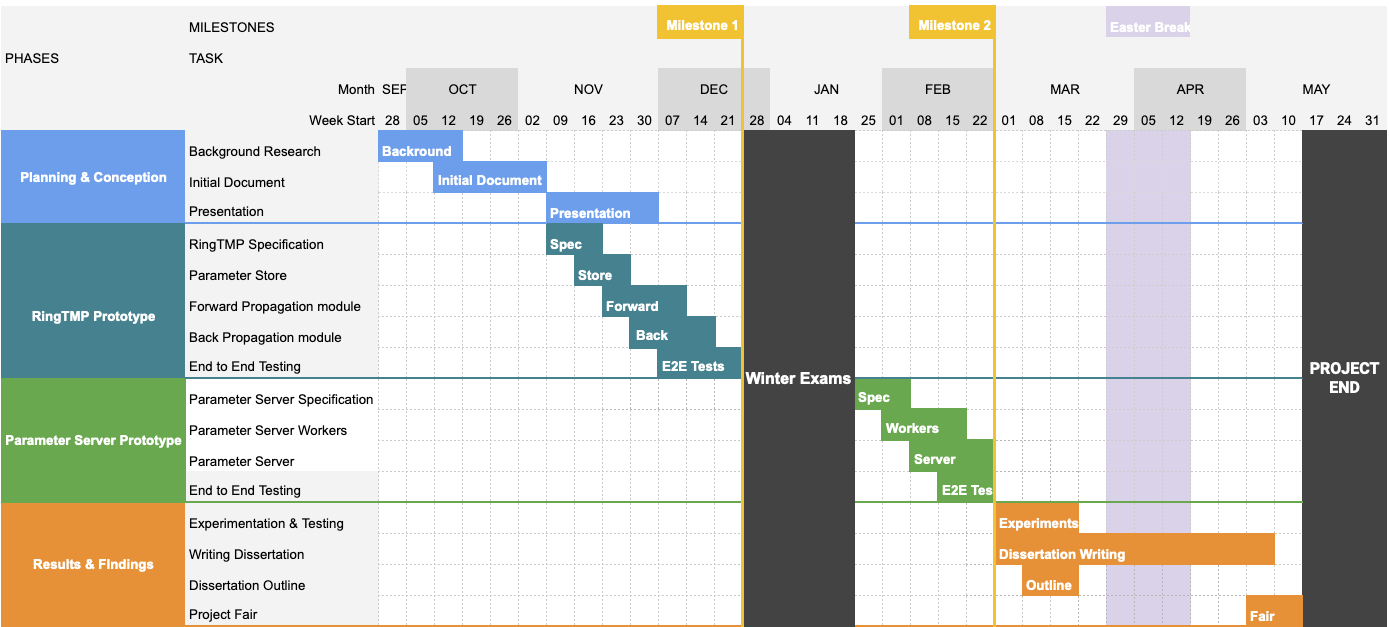
\includegraphics[width=16cm, height=8cm]{BetterGant.png}

The Gantt chart above outlines the order and time frame each task should take in
order complete this dissertation on time and to a high quality. Building a
RingTMP prototype of my system is the most important task to embark on. It is
better to do this first as it will take the longest time to produce and has the
most 'unknown unknowns', moreover this is the centrepiece of my project, if I
have not finished this there will be no dissertation to write. I then take a
month break to revise for my exams. I acknowledge that this is a long time,
however the semester 1 modules contribute more to my final grade than my
dissertation does, therefore its important this project isn't detrimental to my
grades in other modules. After Christmas I'll start work on a basic prototype of
a parameter server. This will use the same tools and languages as my framework.
In this way it will be easy to compare and contrast the benefits and
shortcomings of each system on a level playing field. Once both pieces of
software have been complete I will run various tests to see how well my aims
have been achieved. While I'm conducting these tests I shall also be writing up
my results. Once my experiments have finished I shall start working on my
dissertation document in earnest. I'll hand in my outline a week before easter
break and shall keep working till it is complete.

\subsection{Software Life Cycle}

The methodology I will use to produce my software will be a variation of
Agile methodology. Generally speaking Agile software development models tend to take
the form of doing a small amount of specification upfront and thereafter working
in small cycles to design, develop, validate and deploy a new version of
software. Agile development places particular focus on showing customers working
versions of the software as early as possible an being able to adapt to changing
customer requirements easily. \cite{fowler2001agile}
However the pure Agile methodology does not completely suit my needs, as Agile
programming is customer focused and my project is not. Agile programming also
focuses on changing customer requirements. However there will be no changing
requirements from a customer as there is none. On the other hand optimising for
working software over small iterations is a good philosophy for my work.
Therefore my methodology will specify work upfront and then follow an agile
workflow with week long iterations. I can do this as I won't be beholden to a
customer. This will mean that I have more of an architectural design roadmap
that if I were following a pure Agile methodology.

I also intend to take this iterative methodology to a smaller scale using Test
Driven Development. \cite{beck2003test} This is a philosophy where you write you
tests before you write your code for each logical block. This means you specify
the code's function before you have written it and you have solid acceptance
criteria for when that piece of code is working. If a piece of code is too
complex to test then that is an indication that your logical block needs to be
broken down into small pieces. This way you end up with highly cohesive but
loosely coupled components, and a high degree of confidence that they work.
When introducing new features that effect existing code you can instantly see
where it is breaking as the tests will fail, saving you valuable debugging time.

\subsection{Research Methodology}
My project lends itself to using an experimental research methodology to collect
my findings, with this in mind is paramount to ensure that my results are taken
is as controlled conditions as possible. I will achieve this by
creating two software prototypes, one is my new novel machine learning
framework, the other is the established parameter server design. I will make
these using the same languages and tools as each other. Only the architecture
will differ, meaning comparisons of the two systems will only reflect the
performance of the respective architectures. On these systems I will conduct a
series of tests. Each of these tests will compare each system to one another and
will correspond to the aims I outlined in the introduction:
\begin{itemize}
    \item To compare the efficiency of the systems we can measure the idle time
    of each worker in each of the systems and divide that by the time each
    system took to train a model on some basic task. This will give us a
    percentage of how much time the machine spend processing and how much time
    was spent on communication between nodes. This same experiment can be
    repeated with a different amount of nodes to see how the results change.
    \item To compare the progress made per iteration, the loss function can be
    measured for each iteration in both of the systems, then it is
    straightforward to see which ones makes the most progress.
    \item To measure scalability both systems can be run with a varying number
    of different nodes. In all experiments they are given the same dataset to be
    trained on. We can measure how long it takes for them to complete the task,
    and how well both systems scale when more nodes are added.
    \item To measure resilience a node can be permanently or temporarily removed
    from each system while a model is being trained. Then the success of its
    mitigation and recovery strategies can be assessed.
    \item To discover the limits of how large a neural network each system can
    hold. Tests which incrementally increase the amount of layers and number of
    layers until the system crashes can be run.
\end{itemize}
By doing all this I can measure the performance between these two systems and
accurately assess my architecture's performance relative to the parameter server.

\subsection{Risk Assessment}

A dissertation is a long arduous process in which many things could go wrong.
Hence it is best to identify possible hazards and decide how to mitigate them
before they happen, whilst also having a contingency plan should anything occur. \par

\noindent \textbf{Risk:} The RingTMP prototype is not finished due to time constraints.\\
\textbf{Likelihood:} Low\\
\textbf{Potential Impact:} Severe Impact on the grade for my dissertation.\\
\textbf{Mitigation:} I have thoroughly researched the tools and algorithms I need to
complete this prototype and am familiar with them. This is the first task I will
start work on. Meaning that I have the most time to complete it.\\
\textbf{Contingency Plan:} If I need more time I can reduce the scope of tasks further
down the project timeline. \par

\noindent \textbf{Risk:} Winter exams interfere with my project timeline.\\
\textbf{Likelihood:} Low\\
\textbf{Potential Impact:} The project becomes behind schedule\\
\textbf{Mitigation:} The Winter exams have been factored into the project timeline,
ensuring that I have enough time to revise and keep the project on schedule.\par

\noindent \textbf{Risk:} Parameter Server more complex than initially believed.\\
\textbf{Likelihood:} Medium\\
\textbf{Potential Impact:} The Project becomes behind schedule\\
\textbf{Mitigation:} I have read many papers on the operations of the parameter server
and by being aware with its inner workings. Open source versions of the
parameter server can be found that I can use as a template for my own.\\
\textbf{Contingency Plan:} If the task of creating the parameter server was greatly
underestimated, then an open source version could be used though this would have
repercussions for the meaningfulness of my findings.\par

\noindent \textbf{Risk:} I contract Coronavirus\\
\textbf{Likelihood:} Medium\\
\textbf{Potential Impact:} I have to rest for a number of days, and possibly
have lasting symptoms for months after. \cite{Sudre2020LongCorona}\\
\textbf{Mitigation:} By not returning physically to university, I reduce the
probability of catching Coronavirus, as the cases are much lower in my current
location. My physical social contact will also be kept to a minimum and good hygiene
will be observed\\
\textbf{Contingency Plan:} I will have to isolate for 10 days after displaying
symptoms. For the majority of tasks can be completed in isolation. If I am still
exhibiting symptoms such as fatigue, cognitive impairment and breathlessness I may
have to reassess the scope of the project and apply for extenuating circumstances.\par







% \begin{landscape}
% \begin{tabular}{|l|l|l|l|l|}
% \hline
% Risk                                                                                                       & Likelihood & Potential Impact                                                                                & Mitigation                                                                                                                                                                                                                                                      & Contingency Plan                                                                                                                                                                                                                             \\ \hline
% \begin{tabular}[c]{@{}l@{}}The RingTMP prototype \\ is not finished due\\ to time constraints\end{tabular} & Low        & \begin{tabular}[c]{@{}l@{}}Servere Impact\\ on the grade for\\ my dissertation\end{tabular}     & \begin{tabular}[c]{@{}l@{}}I have thoroughly researched the tools and algorithms\\ I need to complete this prototype and am familiar\\ with them. This is the first task I will start work on.\\ Meaning that I have the most time to complete it.\end{tabular} & \begin{tabular}[c]{@{}l@{}}If I need more time I can reduce the scope of tasks\\  further down the project timeline.\end{tabular}                                                                                                            \\ \hline
% \begin{tabular}[c]{@{}l@{}}Winter exams interfere\\ with my project timeline\end{tabular}                  & Medium     & \begin{tabular}[c]{@{}l@{}}The project\\ becomes behind\\ schedule\end{tabular}                 & \begin{tabular}[c]{@{}l@{}}The Winter exams have been factored into\\ the project timeline, endusuring that I have enough\\ time to revise and keep the prodect on schedule.\end{tabular}                                                                       & Not applicable                                                                                                                                                                                                                               \\ \hline
% \begin{tabular}[c]{@{}l@{}}Parameter Server more\\ complex than initially\\ believed\end{tabular}          & Medium     & \begin{tabular}[c]{@{}l@{}}The project\\ becomes behind\\ schedule\end{tabular}                 & \begin{tabular}[c]{@{}l@{}}I have read many papers on the operations of the\\ parameter server and by being aware with its inner workings.\\ Open source versions of the parameter server can be\\ found that I can use as a template for my own.\end{tabular}  & \begin{tabular}[c]{@{}l@{}}If the task of creating the parameter server was\\ greatly underestimated, then an open source version\\ could be used thoug this would have repercussions\\ for the meaningfullness of my finidngs.\end{tabular} \\ \hline
% I contract Coronavirus                                                                                     & Medium     & \begin{tabular}[c]{@{}l@{}}I have to rest for\\ a number of days\end{tabular}                   & \begin{tabular}[c]{@{}l@{}}By not returning physically to university, I reduce the probability\\ of catching Coronavirus, as the cases are much lower in my\\ current location. My physical social will also be kept to a minimum.\end{tabular}                 & \begin{tabular}[c]{@{}l@{}}I will have to isolate for 10 days after displaying\\ symptoms. For the majority of tasks can be completed\\ in isolation\end{tabular}                                                                            \\ \hline
% \begin{tabular}[c]{@{}l@{}}I catch Coronavirus\\ and exhibit extended\\ sytmptoms\end{tabular}             & Low        & \begin{tabular}[c]{@{}l@{}}The rate at which\\ I can complete\\ my work is limited\end{tabular} & See above.                                                                                                                                                                                                                                                      & \begin{tabular}[c]{@{}l@{}}I will have to reduce the scope of my project, reducing\\ the aims I can deliver on, this will reduce experimentation\\ time and the time it will take to write my disseration.\end{tabular}                      \\ \hline
% \end{tabular}
% \end{landscape}  


